In this section we shall see that \textsc{EviL} is not compact.  This
shall be done by giving an example of an infinite set of formulae for which every finite subset is satisfiable, while the entirety is not.

\begin{lemma}
Let $\tau : \Phi \to \mathcal{L}$ be defined as follows:
\begin{center}
\begin{minipage}{3in}
\begin{tabbing}
	$\tau(p) := $ \=$p \wedge \Pos\top \wedge$ \\
	\> $\Nec$ \= $(\neg p \wedge \Pos\top \wedge$\\
	\> \> $\Nec$ \= $(p \wedge \Pos p))$
\end{tabbing}
\end{minipage}
\end{center}
Every finite subset of $\tau[\Phi]$ is satisfiable, but not the entirety, which is infinite. 
\end{lemma}
\begin{proof}
That $\tau[\Phi]$ is infinite is immediate, as $\Phi$ was stipulated to be infinite. 

So let $S\subseteq \tau[\Phi]$ be finite.  I shall provide a model that
satisfies $S$.  First observe that there is a
 finite $\Psi\subset
\Phi$ such that $S = \tau[\Psi]$.  Let $\{q,r,s\} \subseteq \Phi \; \bs
\; \Psi$ contain
 three distinct letters - this can be done, since $\Phi \;
\bs \; \Psi$ is infinite.
  Let $\mathfrak{M} := \{\pr{a}{\{q\}},
\pr{b}{\{r\}}, \pr{c}{\{s\}} \}$, where 
\begin{align*}
a & := \Psi \cup \{s\} \\
b & := \{q \} \\
c & := \Psi \cup \{r\}
\end{align*}
 Using the same visualization convention I introduced in \S\ref{contradictions},
 $\mathfrak{M}$ can  be visualized% \footnote{I feel I should alert the reader to the fact that I am
   % not employing Kripke  semantics.  The means in which one world 
   % accesses another is not by an accessibility relation, 
   % but rather through the sets of beliefs,
   % which in this case are the sets ${q},{r},$ and ${s}$.} 
in Fig. \ref{fig:mod4}.  It is straightforward to 
check that $\mathfrak{M},( a,\{q\}) \VDash \tau(p)$ for all $p \in \Psi$.

	\begin{figure}[htbp] %  figure placement: here, top, bottom, or page
   \centering
    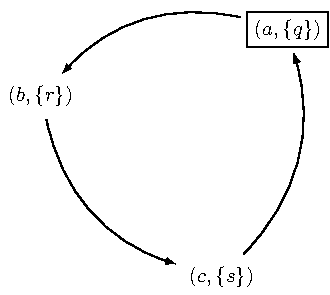
\includegraphics[]{compactness/compactness.pdf}
\caption{$\mathfrak{M},\pr{a}{\{q\}}\VDash \tau[\Psi]$}
   \label{fig:mod4}
\end{figure}
On the other hand, suppose there was some model $\mathfrak{N}$ such that $\mathfrak{N}, ( a, A) \VDash \tau(p)$ for all $p \in \Psi$.
This implies that $\mathfrak{N}, ( a, A) \VDash p$ for each $p \in
\Phi$.  Moreover, let $( b, B)\in\mathfrak{N}$ be such that $b \models A$ 
(one exists since by hypothesis $\mathfrak{N}, ( a, A)
\VDash \Pos p$).  By the semantics of $\tau(p)$, it is evident that
$\mathfrak{N}, ( b, B) \VDash \neg p$ and that there's a $( c, C)\in\mathfrak{N}$
such that $c \models B$ and $\mathfrak{N},( c,C )
\VDash p \wedge \Pos p$.  But then from this it must be that $a$ and
$c$ both contain exactly the same sentence letters, so $a = b$ which means that
$a \models B$ as well, since $B \subseteq
\mathcal{L}_0$ (as per the grammar restriction).  However it cannot be that
$\mathfrak{N},( a,A ) \VDash \Pos p$ since $\mathfrak{N},( a,A )
\VDash \Nec \neg p$, which follows from the assumption that $\mathfrak{N},( a,A )
\VDash \tau(p)$. 
Thus it is impossible that $\mathfrak{N},( a, A) \VDash \tau[\Phi]$. $\lightning$
\end{proof}

The above argument illustrates that while \textsc{EviL} semantics
present themselves as similar to the traditional Kripke Semantics for modal
logic, they aren't the same.  The similarity particularly manifests
itself when thinking about visualizations like Fig. \ref{fig:mod4}.
But if for some reason two world-pairs $(a,A)$ and $(b,B)$ make true
the same sentence letters, then $a=b$.
Moreover, for any $C \subseteq \mathcal{L}_0$, we have that $a \models
C$ if and only if $b \models C$ in this case. This is crucial - even though
\textsc{EviL} is modal, it has no accessibility relations; the role of
accessibility relations is instead picked up by basic sets of beliefs
$C$.
It is necessarily the case that for a basic set of beliefs $C$ that
$C\subseteq \mathcal{L}_0$, due to grammar restriction I decided upon
to ensure the semantics of \textsc{EviL} were well-defined.
It is from this basic design choice that my unusual failure of compactness manifests itself.
I shall return to considering the relationship of Kripke semantics and
\textsc{EviL} models in \S\ref{kripke}.

The failure of compactness, while a fairly basic result in the model
theory of \textsc{EviL}, is far reaching.  As a consequence, there is
no hope of achieving completeness using infinitary Lindenbaum
constructions that are typically employed in modal logic, such as is
done in \citep[][chapter 4]{blackburn_modal_2001}, for instance.
Hence the completeness theorem for \textsc{EviL} presented in \S\ref{army-of-darkness}
will necessarily have to be finite in nature.
%%% Local Variables: 
%%% mode: latex
%%% TeX-master: "evil_philosophy"
%%% End: 
